%%%%%%%%%%%%%%%%%%%%%%%%%%%%%%%%%%%%%%%%%
% Guide Book (Documentation Template)
% LaTeX Template
% Version 1.0 (20/10/16)
%
% This template has been downloaded from:
% http://www.LaTeXTemplates.com
%
% Original author:
% Francisco Maria Calisto
%
% License:
% Apache License (Version 2.0)
%
% IMPORTANT NOTE:
% In addition to running BibTeX to compile the reference list from the .bib
% file, you will need to run MakeIndex to compile the index at the end of the
% document.
%
%%%%%%%%%%%%%%%%%%%%%%%%%%%%%%%%%%%%%%%%%

%------------------------------------------------------------------------------
%	PACKAGES AND OTHER DOCUMENT CONFIGURATIONS
%------------------------------------------------------------------------------

\documentclass{tufte-book} % Use the tufte-book class which in turn uses the tufte-common class

\usepackage{graphicx}
\graphicspath{ {graphics/} }

% encoding
%--------------------------------------
\usepackage[utf8]{inputenc}
\usepackage[T1]{fontenc}
%--------------------------------------
 
% Portuguese-specific commands
%--------------------------------------
\usepackage[portuguese]{babel}
%--------------------------------------

% Uncomment this line if you prefer colored hyperlinks
% (e.g., for onscreen viewing)
%--------------------------------------
\hypersetup{colorlinks}
%--------------------------------------

%%
% Book metadata
\title{Guia Balsamiq\\(PT)}
\author[Professor]{Francisco Maria Calisto}
\publisher{Usabilidade e Sistemas de Informação}

%%
% If they're installed, use Bergamo and Chantilly from www.fontsite.com.
% They're clones of Bembo and Gill Sans, respectively.
%\IfFileExists{bergamo.sty}{\usepackage[osf]{bergamo}}{}% Bembo
%\IfFileExists{chantill.sty}{\usepackage{chantill}}{}% Gill Sans

%\usepackage{microtype}

%%
% Just some sample text
\usepackage{lipsum}

%%
% For nicely typeset tabular material
\usepackage{booktabs}

%%
% For graphics / images
\usepackage{graphicx}
\setkeys{Gin}{width=\linewidth,totalheight=\textheight,keepaspectratio}
\graphicspath{{graphics/}}

% The fancyvrb package lets us customize the formatting of verbatim
% environments.  We use a slightly smaller font.
\usepackage{fancyvrb}
\fvset{fontsize=\normalsize}

%%
% Prints argument within hanging parentheses (i.e., parentheses that take
% up no horizontal space).  Useful in tabular environments.
\newcommand{\hangp}[1]{\makebox[0pt][r]{(}#1\makebox[0pt][l]{)}}

%%
% Prints an asterisk that takes up no horizontal space.
% Useful in tabular environments.
\newcommand{\hangstar}{\makebox[0pt][l]{*}}

%%
% Prints a trailing space in a smart way.
\usepackage{xspace}

%%
% Some shortcuts for Tufte's book titles.  The lowercase commands will
% produce the initials of the book title in italics.  The all-caps commands
% will print out the full title of the book in italics.
\newcommand{\vdqi}{\textit{VDQI}\xspace}
\newcommand{\ei}{\textit{EI}\xspace}
\newcommand{\ve}{\textit{VE}\xspace}
\newcommand{\be}{\textit{BE}\xspace}
\newcommand{\VDQI}{\textit{The Visual Display of Quantitative Information}\xspace}
\newcommand{\EI}{\textit{Envisioning Information}\xspace}
\newcommand{\VE}{\textit{Visual Explanations}\xspace}
\newcommand{\BE}{\textit{Beautiful Evidence}\xspace}

\newcommand{\TL}{Tufte-\LaTeX\xspace}

% Prints the month name (e.g., January) and the year (e.g., 2008)
\newcommand{\monthyear}{%
  \ifcase\month\or January\or February\or March\or April\or May\or June\or
  July\or August\or September\or October\or November\or
  December\fi\space\number\year
}


% Prints an epigraph and speaker in sans serif, all-caps type.
\newcommand{\openepigraph}[2]{%
  %\sffamily\fontsize{14}{16}\selectfont
  \begin{fullwidth}
  \sffamily\large
  \begin{doublespace}
  \noindent\allcaps{#1}\\% epigraph
  \noindent\allcaps{#2}% author
  \end{doublespace}
  \end{fullwidth}
}

% Inserts a blank page
\newcommand{\blankpage}{\newpage\hbox{}\thispagestyle{empty}\newpage}

\usepackage{units}

% Typesets the font size, leading, and measure in the form of 10/12x26 pc.
\newcommand{\measure}[3]{#1/#2$\times$\unit[#3]{pc}}

% Macros for typesetting the documentation
\newcommand{\hlred}[1]{\textcolor{Maroon}{#1}}% prints in red
\newcommand{\hangleft}[1]{\makebox[0pt][r]{#1}}
\newcommand{\hairsp}{\hspace{1pt}}% hair space
\newcommand{\hquad}{\hskip0.5em\relax}% half quad space
\newcommand{\TODO}{\textcolor{red}{\bf TODO!}\xspace}
\newcommand{\ie}{\textit{i.\hairsp{}e.}\xspace}
\newcommand{\eg}{\textit{e.\hairsp{}g.}\xspace}
\newcommand{\na}{\quad--}% used in tables for N/A cells
\providecommand{\XeLaTeX}{X\lower.5ex\hbox{\kern-0.15em\reflectbox{E}}\kern-0.1em\LaTeX}
\newcommand{\tXeLaTeX}{\XeLaTeX\index{XeLaTeX@\protect\XeLaTeX}}
% \index{\texttt{\textbackslash xyz}@\hangleft{\texttt{\textbackslash}}\texttt{xyz}}
\newcommand{\tuftebs}{\symbol{'134}}% a backslash in tt type in OT1/T1
\newcommand{\doccmdnoindex}[2][]{\texttt{\tuftebs#2}}% command name -- adds backslash automatically (and doesn't add cmd to the index)
\newcommand{\doccmddef}[2][]{%
  \hlred{\texttt{\tuftebs#2}}\label{cmd:#2}%
  \ifthenelse{\isempty{#1}}%
    {% add the command to the index
      \index{#2 command@\protect\hangleft{\texttt{\tuftebs}}\texttt{#2}}% command name
    }%
    {% add the command and package to the index
      \index{#2 command@\protect\hangleft{\texttt{\tuftebs}}\texttt{#2} (\texttt{#1} package)}% command name
      \index{#1 package@\texttt{#1} package}\index{packages!#1@\texttt{#1}}% package name
    }%
}% command name -- adds backslash automatically
\newcommand{\doccmd}[2][]{%
  \texttt{\tuftebs#2}%
  \ifthenelse{\isempty{#1}}%
    {% add the command to the index
      \index{#2 command@\protect\hangleft{\texttt{\tuftebs}}\texttt{#2}}% command name
    }%
    {% add the command and package to the index
      \index{#2 command@\protect\hangleft{\texttt{\tuftebs}}\texttt{#2} (\texttt{#1} package)}% command name
      \index{#1 package@\texttt{#1} package}\index{packages!#1@\texttt{#1}}% package name
    }%
}% command name -- adds backslash automatically
\newcommand{\docopt}[1]{\ensuremath{\langle}\textrm{\textit{#1}}\ensuremath{\rangle}}% optional command argument
\newcommand{\docarg}[1]{\textrm{\textit{#1}}}% (required) command argument
\newenvironment{docspec}{\begin{quotation}\ttfamily\parskip0pt\parindent0pt\ignorespaces}{\end{quotation}}% command specification environment
\newcommand{\docenv}[1]{\texttt{#1}\index{#1 environment@\texttt{#1} environment}\index{environments!#1@\texttt{#1}}}% environment name
\newcommand{\docenvdef}[1]{\hlred{\texttt{#1}}\label{env:#1}\index{#1 environment@\texttt{#1} environment}\index{environments!#1@\texttt{#1}}}% environment name
\newcommand{\docpkg}[1]{\texttt{#1}\index{#1 package@\texttt{#1} package}\index{packages!#1@\texttt{#1}}}% package name
\newcommand{\doccls}[1]{\texttt{#1}}% document class name
\newcommand{\docclsopt}[1]{\texttt{#1}\index{#1 class option@\texttt{#1} class option}\index{class options!#1@\texttt{#1}}}% document class option name
\newcommand{\docclsoptdef}[1]{\hlred{\texttt{#1}}\label{clsopt:#1}\index{#1 class option@\texttt{#1} class option}\index{class options!#1@\texttt{#1}}}% document class option name defined
\newcommand{\docmsg}[2]{\bigskip\begin{fullwidth}\noindent\ttfamily#1\end{fullwidth}\medskip\par\noindent#2}
\newcommand{\docfilehook}[2]{\texttt{#1}\index{file hooks!#2}\index{#1@\texttt{#1}}}
\newcommand{\doccounter}[1]{\texttt{#1}\index{#1 counter@\texttt{#1} counter}}

% Generates the index
\usepackage{makeidx}
\makeindex

\begin{document}

% r.3 full title page
\maketitle

% r.5 contents
\tableofcontents

% r.9 introduction
\cleardoublepage
\chapter*{Introdução}

\begin{center}
	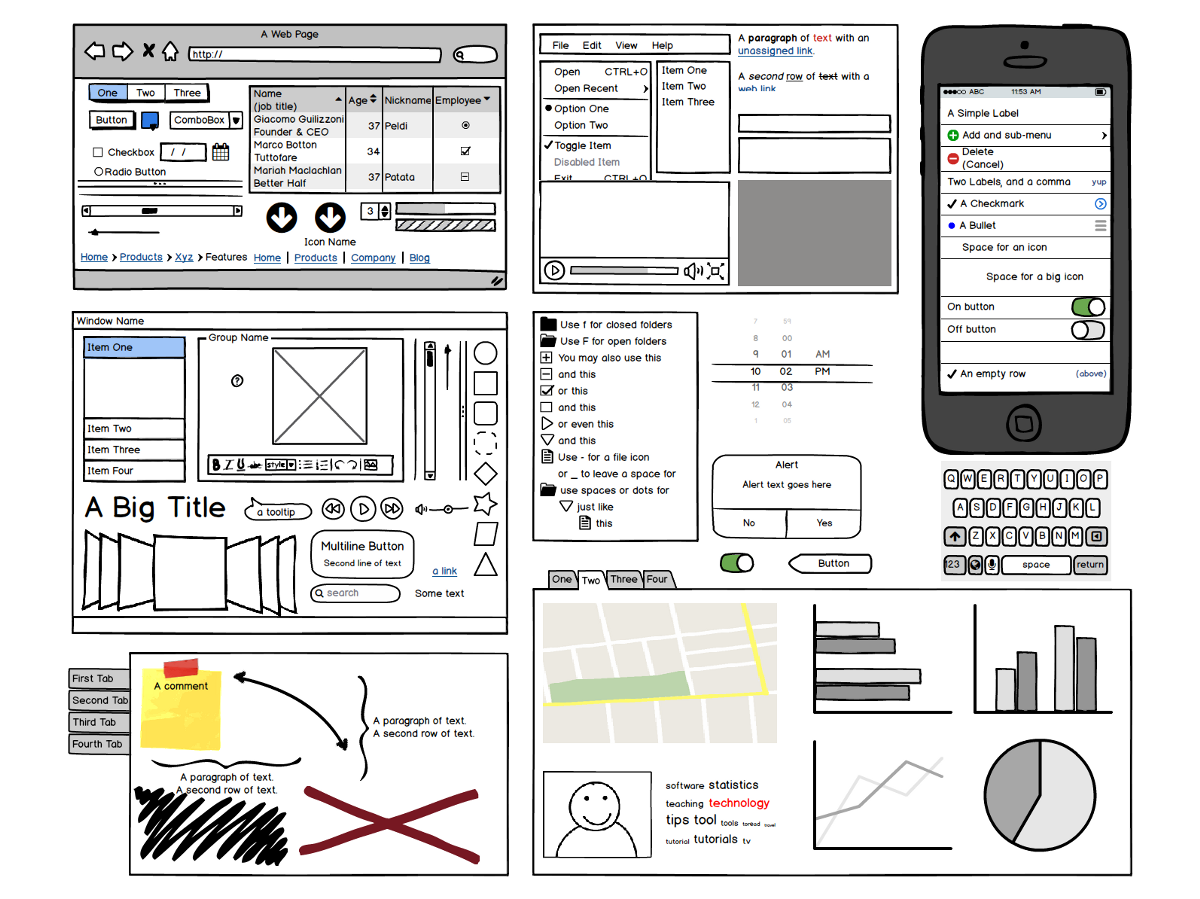
\includegraphics[width=15cm]{img1.png}
\end{center}

O Balsamiq é uma ferramenta de prototipagem rápida e pragmática que pode ser usada para criar wireframes e protótipos de várias aplicações.

Para compreender o Balsamiq é necessário compreender os conceitos de wireframing. Wireframing, é claro, uma forma de esboçar ideias para uma interface de produto ou web, descrevendo a um alto nível o que esta irá fazer, como pode parecer, e como a mesma irá funcionar.

Antes do Balsamiq existiam outras aplicações semelhantes no entanto os modelos de wireframing eram tradicionalmente feitos à mão e em papel, ou usando ferramentas digitais onde os resultados eram semelhantes ao Balsamiq mas mais complexas de usar.

Neste guia serão explicados alguns fundamentos de iniciação ao Balsamiq e como desenvolver um protótipo em wireframing.

%%
% Start the main matter (normal chapters)
\mainmatter

\chapter{Instalação}

Por favor aceda ao \href{https://tecnico.mybalsamiq.com/}{MyBalsamiq} e introduza as suas credenciais.

\begin{center}
	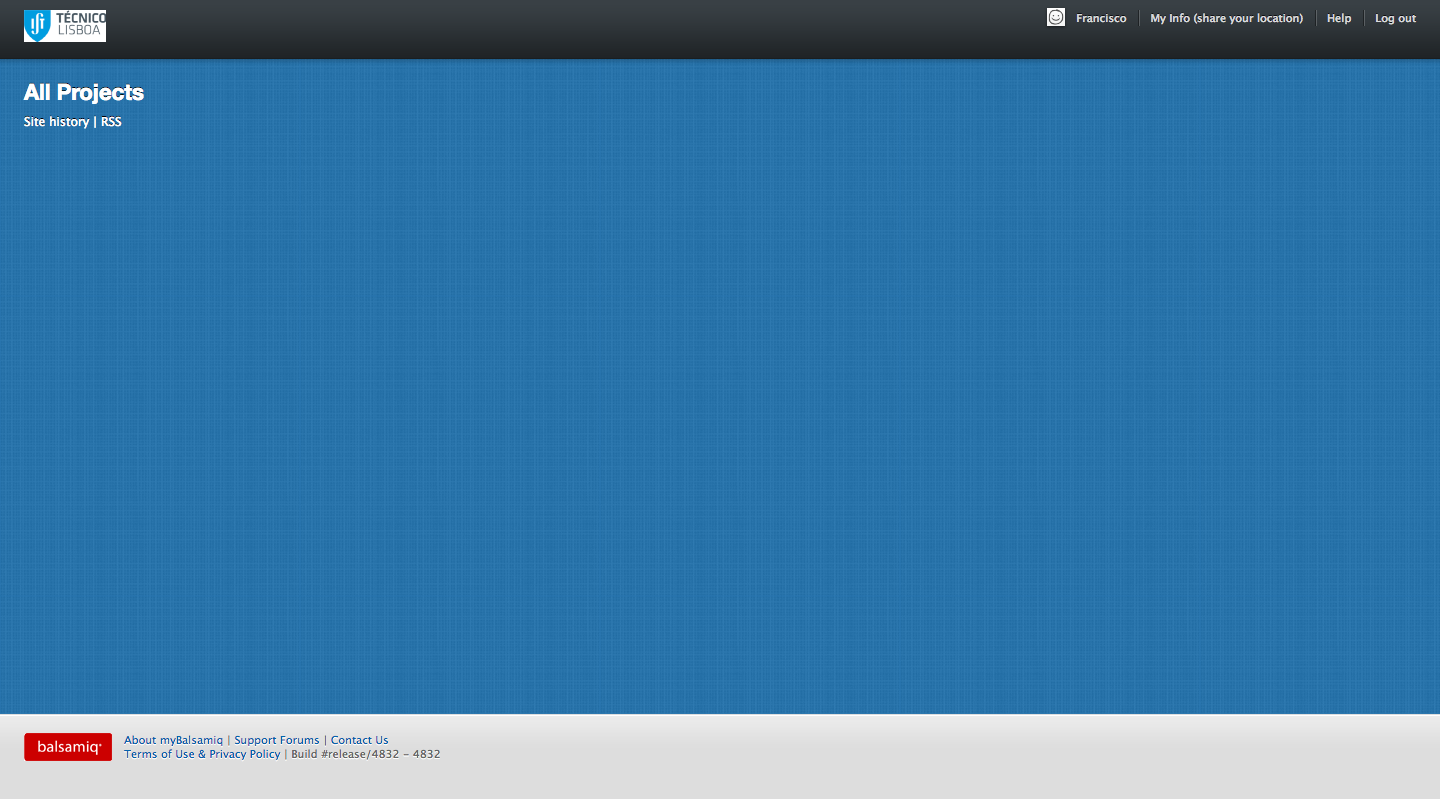
\includegraphics{img25.png}
\end{center}

Ou aceda ao link \href{https://balsamiq.com/}{balsamiq.com} e faça o download da aplicação para Desktop.

\begin{center}
	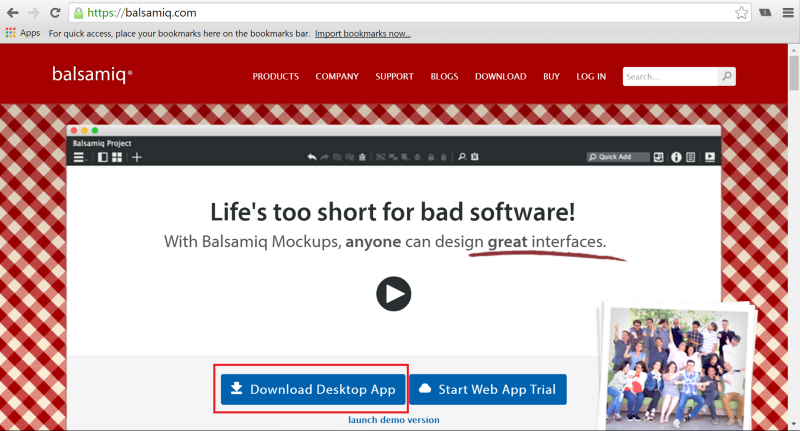
\includegraphics{img2.png}
\end{center}

Este guia será feito para a aplicação Desktop muito semelhante à aplicação em ambiente Web.

\chapter{Criar um Mockup}

\begin{center}
	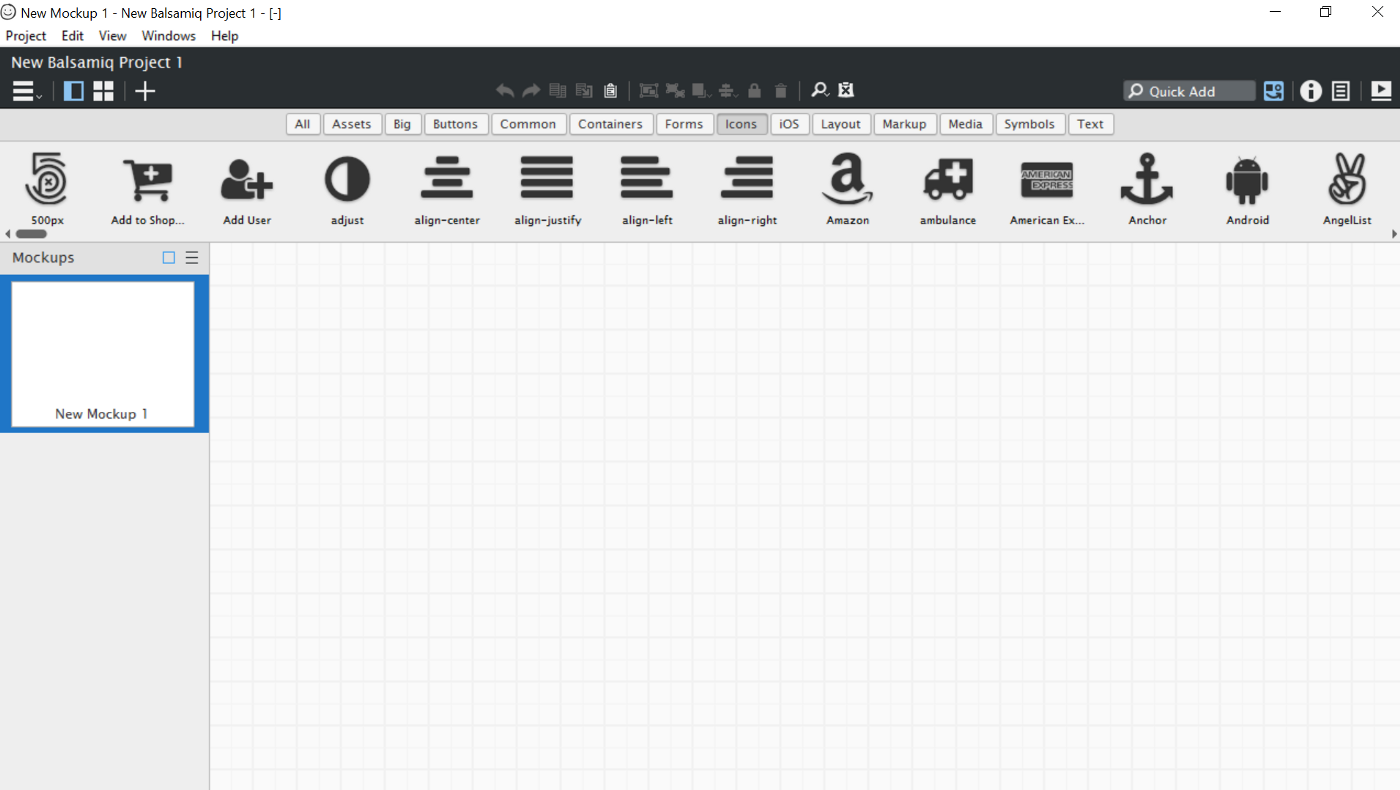
\includegraphics{img3.png}
\end{center}

Esta é a página que verá quando abre o Balsamiq. É um novo projeto em branco.

\begin{center}
	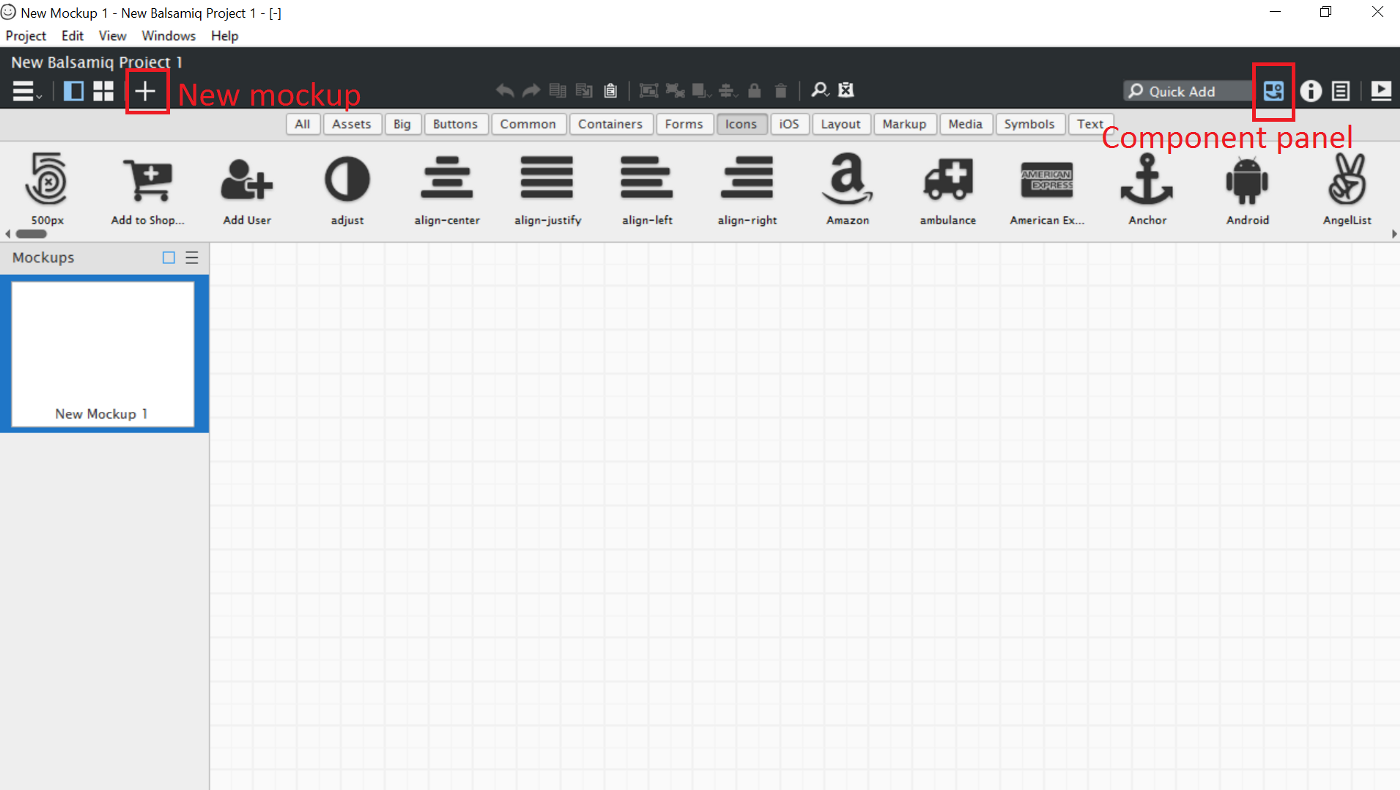
\includegraphics{img4.png}
\end{center}

Uma nova maquete é uma nova vista para a aplicação que irá criar.

Por padrão, terá uma vista em branco aberto. Mas, se quiser vistas adicionais, clique no símbolo + marcado com uma caixa vermelha como pode ver na imagem.

O smiley como ícone no canto superior direito é um atalho para abrir o painel componente onde você vai encontrar todos os seus componentes que usam lata em seu projeto.

\chapter{Recursos da ferramenta}

Existe um ícone de propriedades do projeto no canto superior direito onde pode definir as propriedades gerais do projeto. Tais como, descrição, skin, fontes de letra e cores.

\begin{center}
	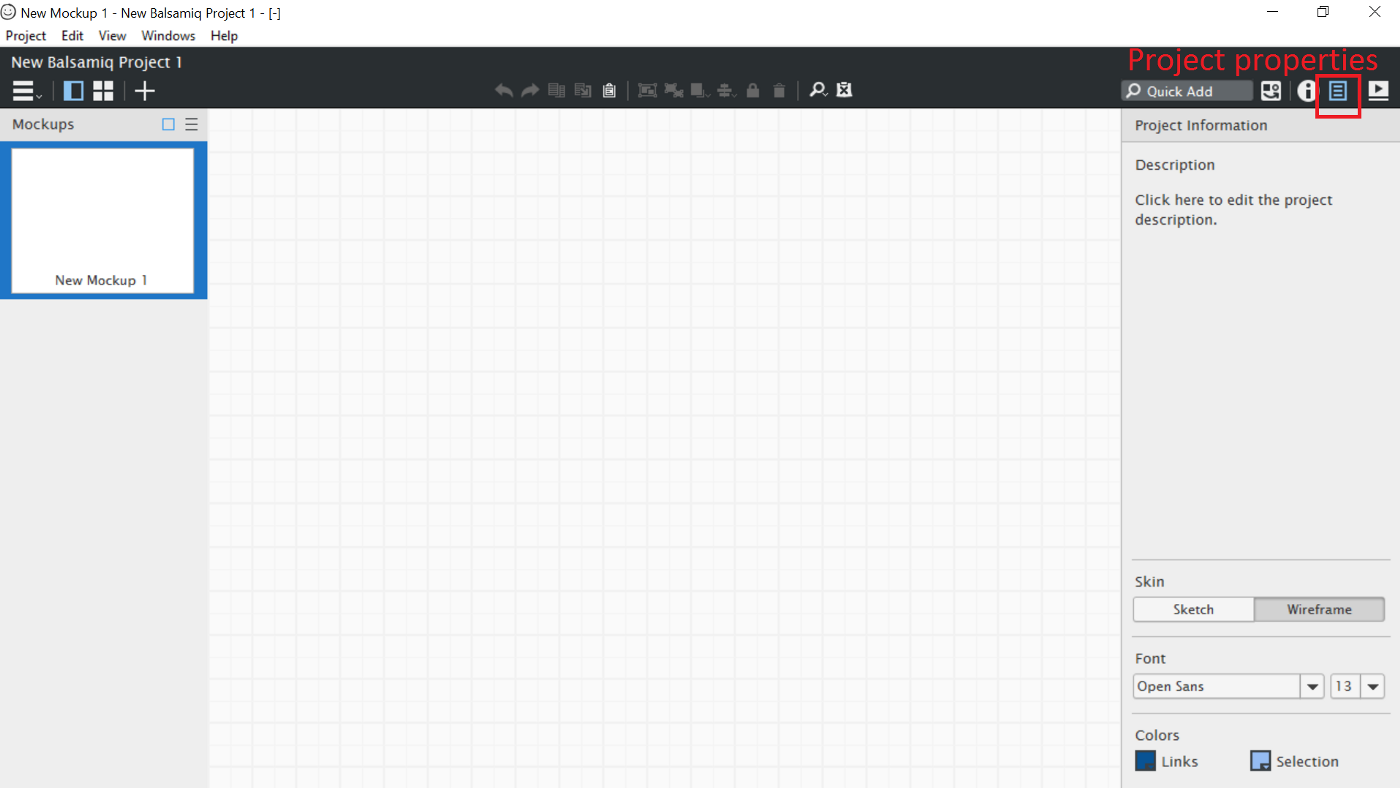
\includegraphics{img5.png}
\end{center}

São dadas duas opções diferentes para a skin do Balsamiq - Sketch e wireframe.

É bastante auto-explicativo.

Sketch dá uma aparência áspera para o protótipo e wireframe parece mais limpo.

\break

Pode ver a diferença entre as duas imagens abaixo:

\begin{center}
	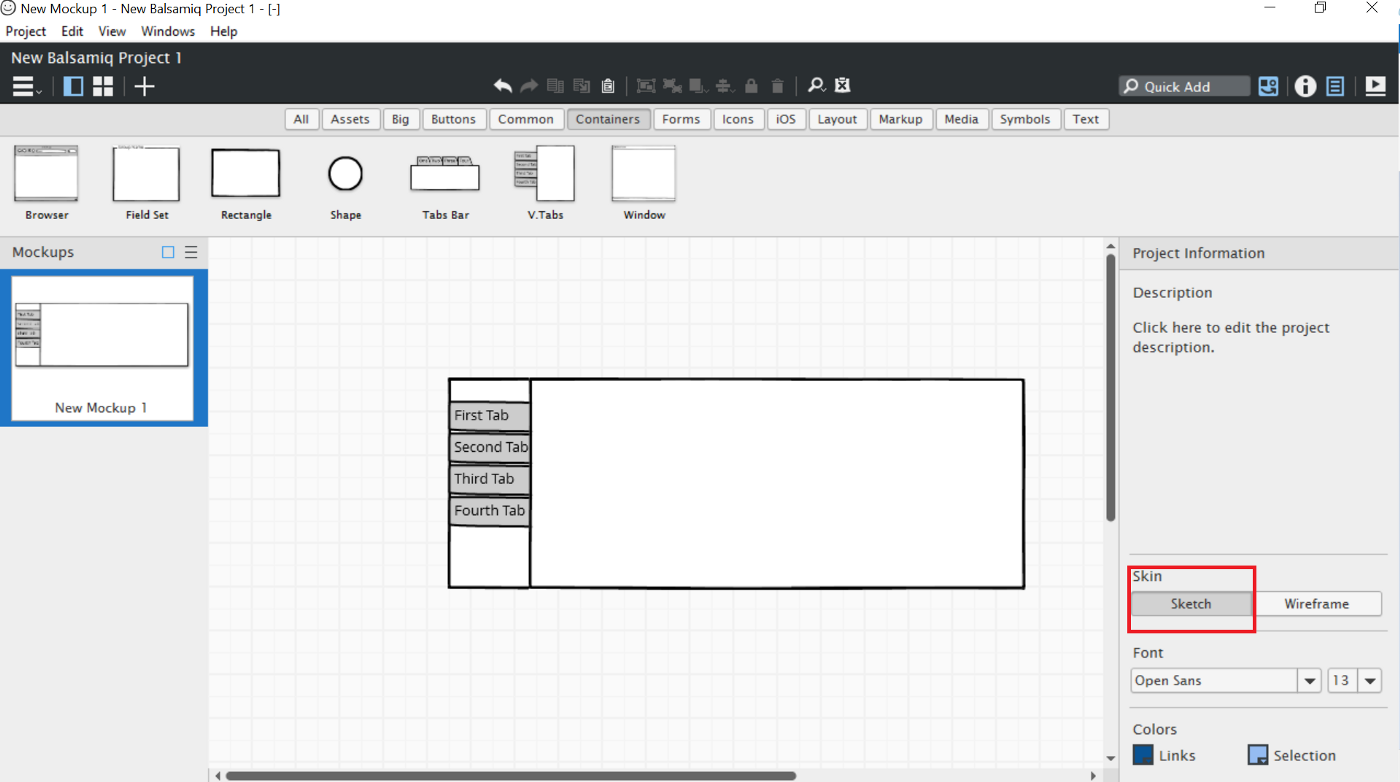
\includegraphics{img6.png}
\end{center}

\begin{center}
	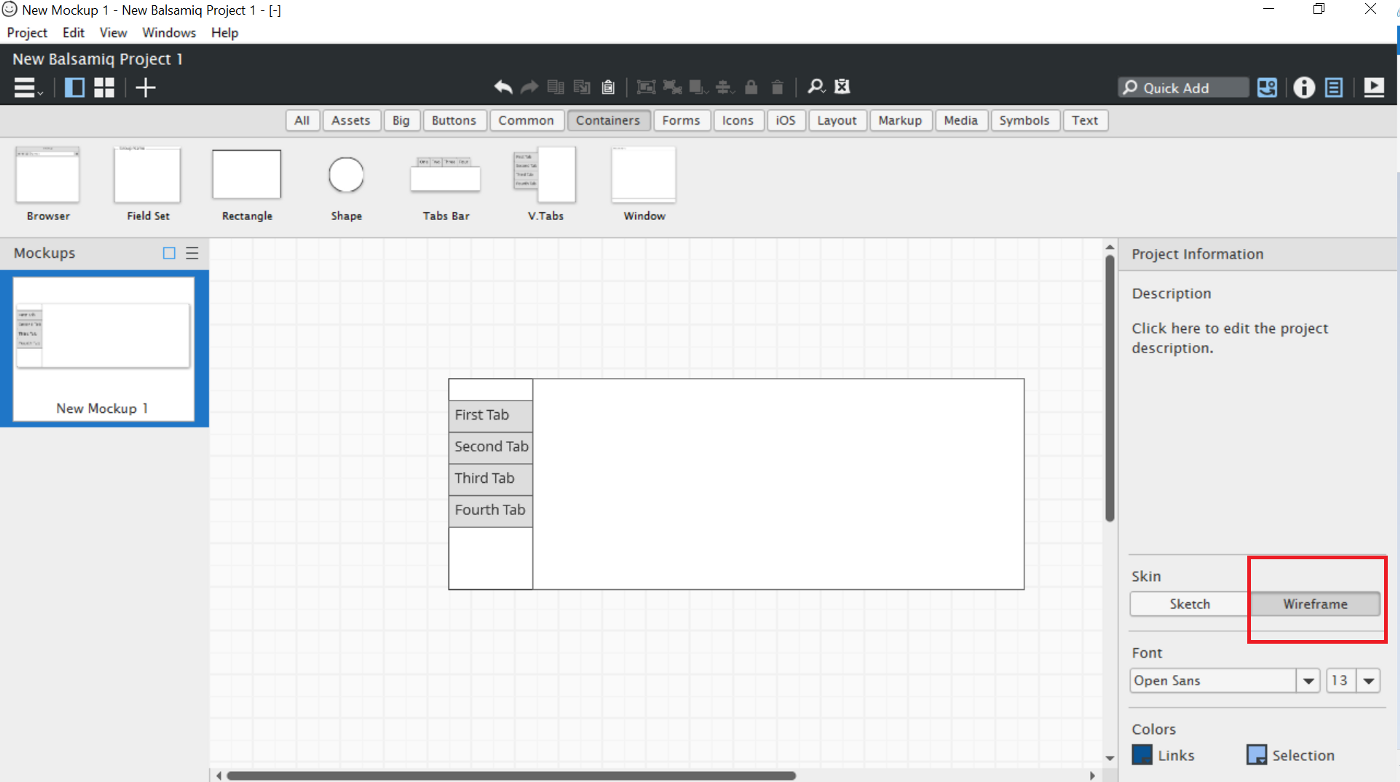
\includegraphics{img7.png}
\end{center}

Pode mudar entre as skins em qualquer ponto no projeto, mas o alinhamento dos componentes pode mudar se alterá-lo mais tarde.

Então, é um bom ponto escolher a skin no inicio de cada projecto.

\begin{center}
	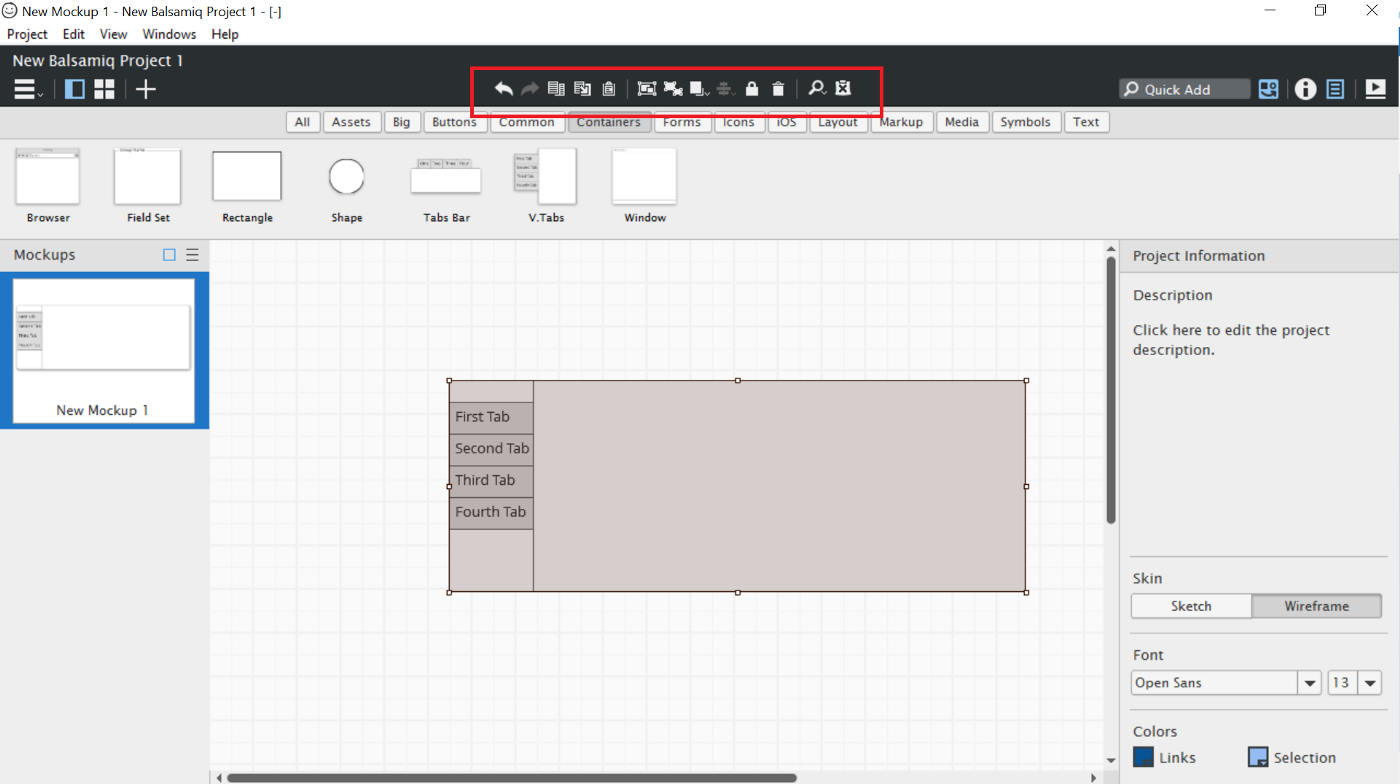
\includegraphics{img8.png}
\end{center}

Ao selecionar qualquer componente da vista actual, um conjunto de ferramentas de edição rápida aparecer em cima do componente.

Da esquerda para a direita, é: reverse, forward, duplicate, copy, paste, group, ungroup, (bring to front, push to back), (align, space out), lock, delete, zoom e hide.

\begin{center}
	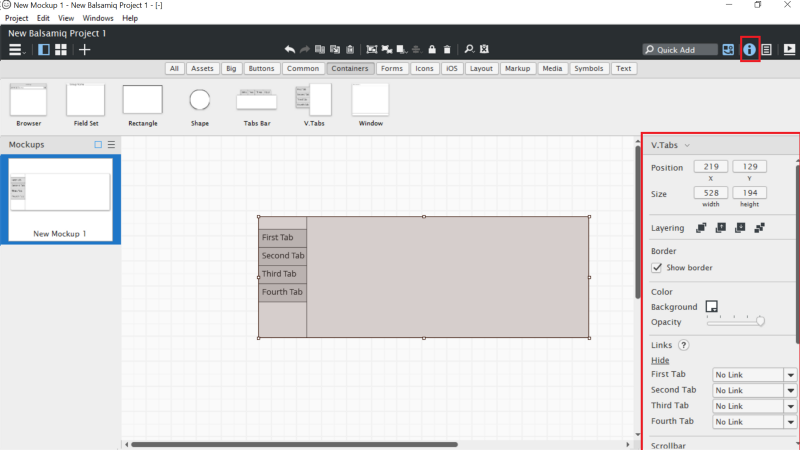
\includegraphics{img9.png}
\end{center}

Agora o ícone da caixa dá-lhe propriedades adicionais para o componente. Tais como definir a altura e largura, a posição, a cor, links e outras propriedades que são específicas para cada componente.

\break

\begin{center}
	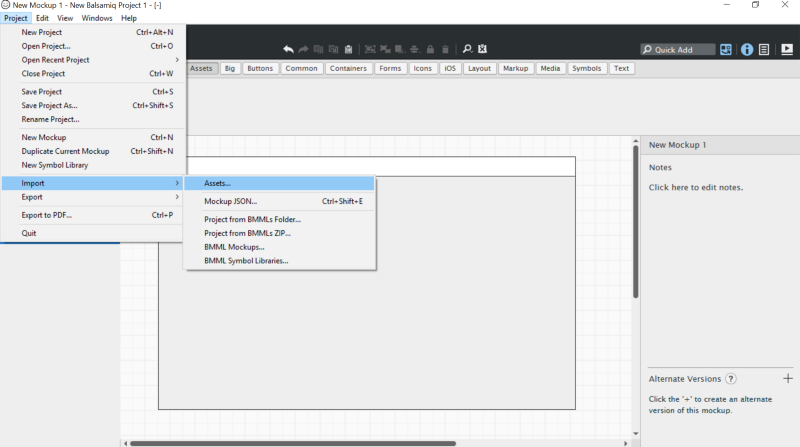
\includegraphics{img10.png}
\end{center}

Se desejar importar uma imagem ou elemento media de externo, pode optar por fazê-lo, selecionando project -> import -> assets  e apenas importá-los.

Aqui vai encontrá-los no separador activo disponível no painel componente.

\chapter{Criar Vistas}

Observe agora com atenção a criação de novas vistas que são fundamentais mais tarde para a fase funcional dos protótipo.

1) Arrastando o componente iPad para a vista:

\begin{center}
	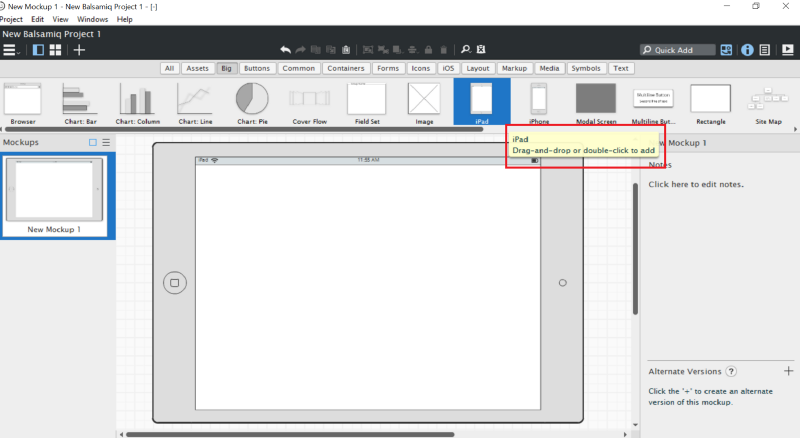
\includegraphics{img11.png}
\end{center}

\break

2) Definir as propriedades para o componente:

\begin{center}
	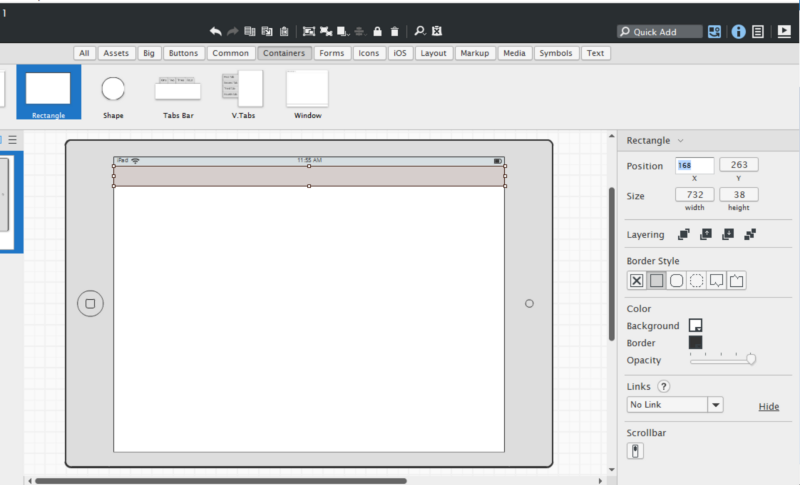
\includegraphics{img12.png}
\end{center}

\break

3) Arrastou um componente da caixa da lista na vista:

\begin{center}
	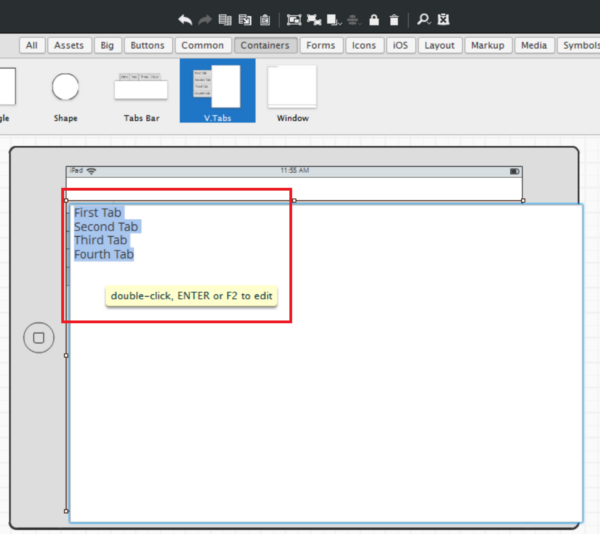
\includegraphics{img13.png}
\end{center}

Para adicionar texto ao componente, clique duas vezes sobre o mesmo e pode também adicionar texto.

Este recurso está disponível em todas as componentes, onde tem o recurso de adicionar texto.

\break

4) Escolha a seleção para o componente no painel de propriedades à direita:

\begin{center}
	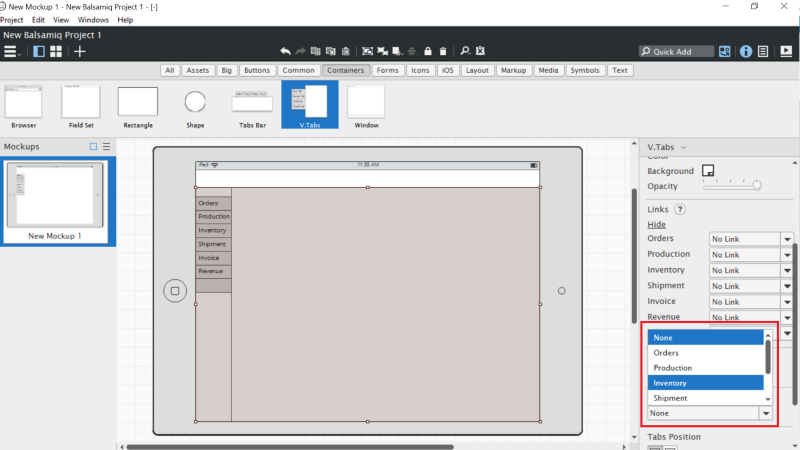
\includegraphics{img14.png}
\end{center}

5) Adicione um componente media (logo):

\begin{center}
	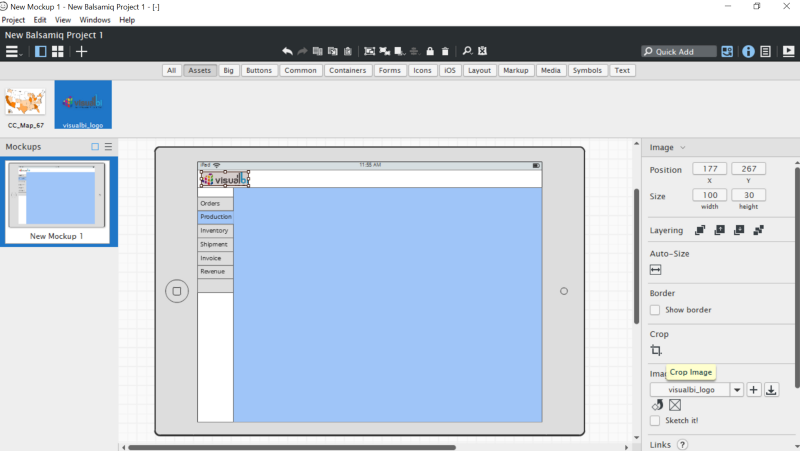
\includegraphics{img15.png}
\end{center}

6) Mude de cor para a caixa das listas e adicione o texto:

\begin{center}
	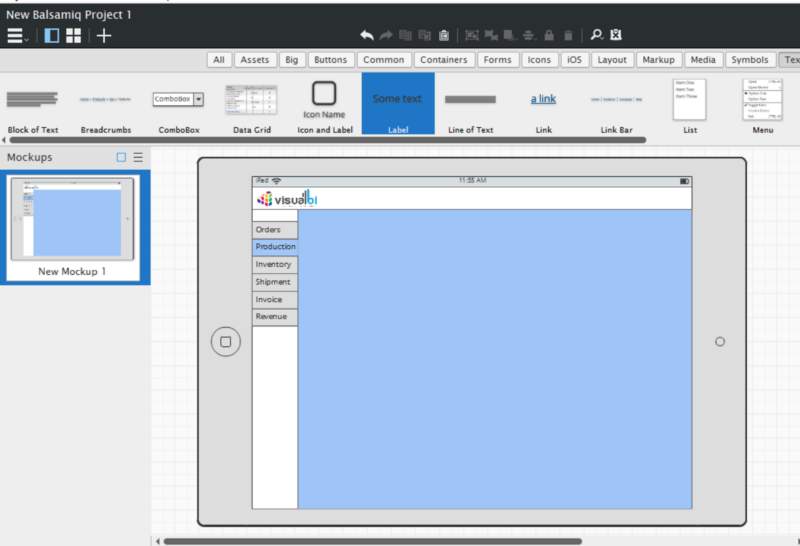
\includegraphics{img16.png}
\end{center}

\break

7) Adicione vários componentes e crie o aplicativo do painel:

\begin{center}
	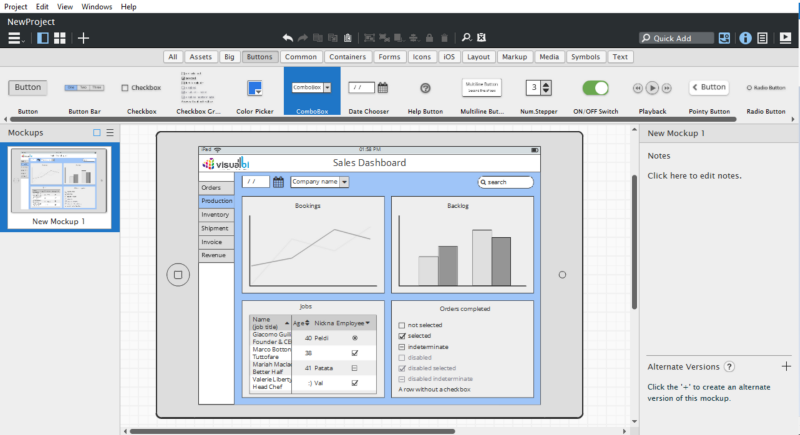
\includegraphics{img17.png}
\end{center}

8) Clique no lado direito sobre maquete e duplique-a para a próxima vista:

\begin{center}
	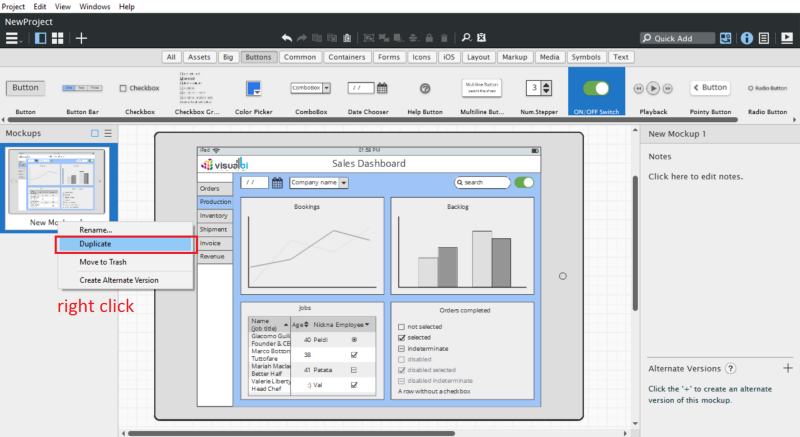
\includegraphics{img18.png}
\end{center}

'Links' são onde pode vincular um componente para outro mockup, endereço web ou voltar se estiver no modo de apresentação.

\begin{center}
	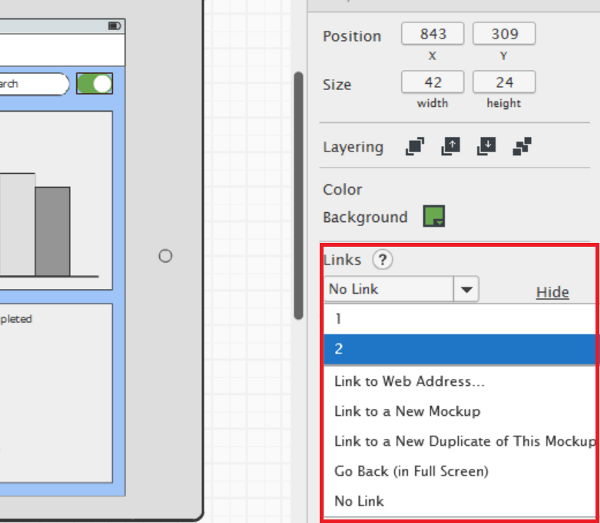
\includegraphics{img19.png}
\end{center}

Desta forma, pode selecionar um componente e, em seguida, clique na opção de link no painel de propriedades para vinculá-lo.

\break

9) O botão de play significa ir para o modo de apresentação:

\begin{center}
	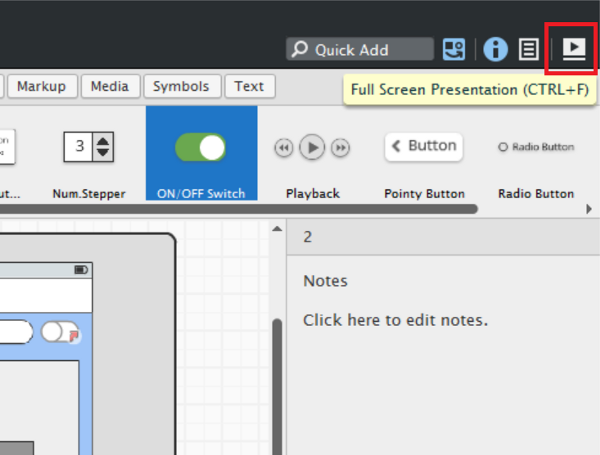
\includegraphics{img20.png}
\end{center}

Qualquer componente que revela um ícone semelhante a uma mão quando passa o ponteiro do rato sobre o mesmo tem um link anexado.

\begin{center}
	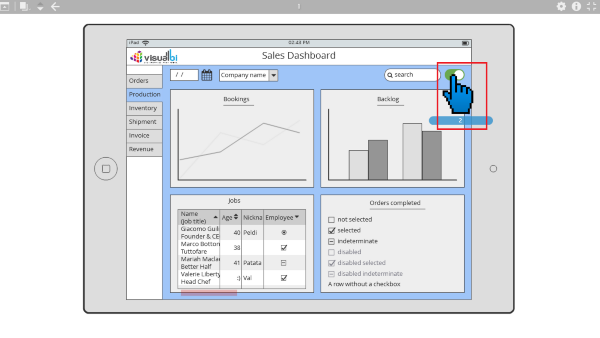
\includegraphics{img21.png}
\end{center}

10) Quando clicou no botão verde de alternância, o botão alterna para revelar uma visualização do mapa:

\begin{center}
	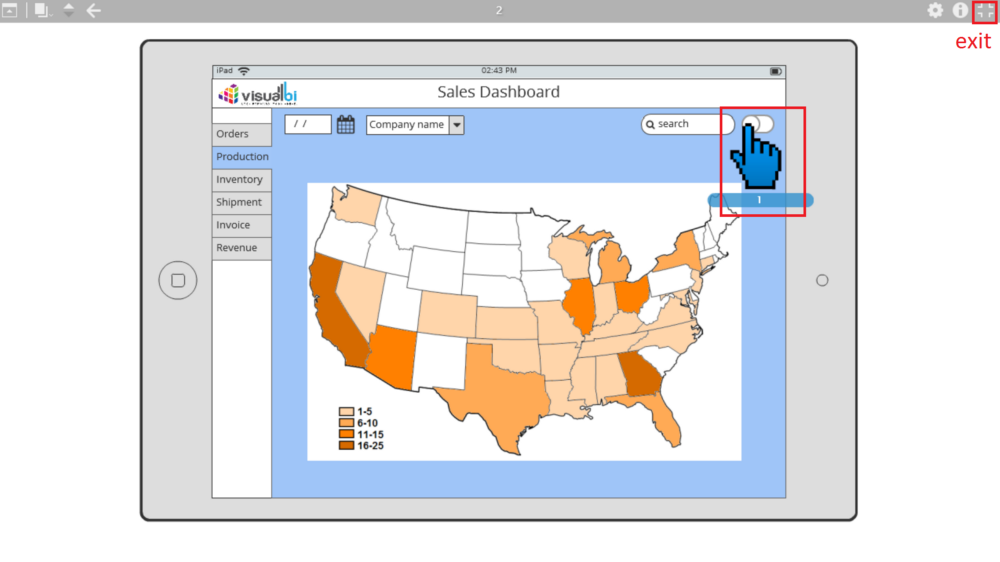
\includegraphics{img22.png}
\end{center}

E o ícone superior direito sai da vista de apresentação.

11) Tem a opção de exportar uma única vista como uma imagem PNG, mas se deseja exportar o projeto como um wireframe clicável interativo, tem a opção de exportá-lo como um PDF:

\begin{center}
	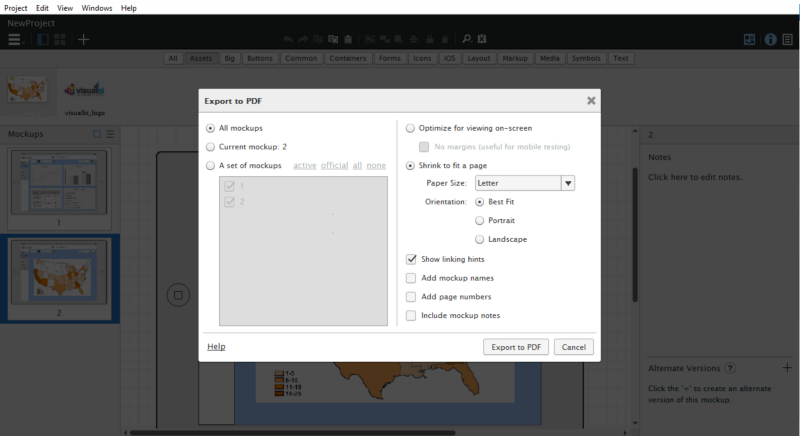
\includegraphics{img23.png}
\end{center}

\begin{center}
	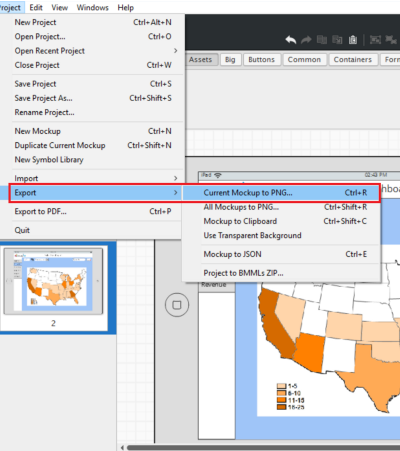
\includegraphics{img24.png}
\end{center}

\chapter{Informações}

%%
% The back matter contains appendices, bibliographies, indices, glossaries, etc.

\backmatter

\bibliography{sample-handout}
\bibliographystyle{plainnat}


\printindex

\end{document}
